\documentclass[11pt,letterpaper]{article}
\usepackage[T1]{fontenc}
\usepackage{lmodern}
\usepackage[margin=1.03in,headheight=14pt]{geometry}
\usepackage{amsmath,amssymb,amsthm,mathtools}
\usepackage{microtype,array,booktabs,xcolor,tikz}
\usepackage{fancyhdr}
\usepackage{hyperref}
\definecolor{inkblue}{HTML}{234D69}
\definecolor{orbitgold}{HTML}{9A5A23}
\definecolor{orbitgreen}{HTML}{276559}
\hypersetup{colorlinks,linkcolor=inkblue,citecolor=inkblue,urlcolor=inkblue,
  pdftitle={The Sharp Twelve-Point Bound in Mordell's Distance-Product Problem},
  pdfauthor={Fengcan Jiang's Mordell research project},
  pdfkeywords={Mordell problem, distance product, positive semidefinite kernels, interval arithmetic}}
\setcounter{tocdepth}{1}
\setlength{\emergencystretch}{2em}
\pagestyle{fancy}
\fancyhf{}
\fancyhead[L]{\small Mordell's distance-product problem}
\fancyhead[R]{\small The twelve-point theorem}
\fancyfoot[C]{\small\thepage}
\renewcommand{\headrulewidth}{0.3pt}
\newtheorem{theorem}{Theorem}
\newtheorem{lemma}[theorem]{Lemma}
\newtheorem{proposition}[theorem]{Proposition}
\newtheorem{corollary}[theorem]{Corollary}
\theoremstyle{remark}
\newtheorem{remark}[theorem]{Remark}
\newcommand{\CC}{\mathbb C}
\newcommand{\RR}{\mathbb R}
\newcommand{\QQ}{\mathbb Q}
\newcommand{\RePart}{\operatorname{Re}}
\newcommand{\ImPart}{\operatorname{Im}}
\newcommand{\certroot}{\href{https://github.com/harrykane8816627373-cell/mordell-research/tree/3c922f3446f4f32441d75aef1d7907d38b0544f7}{fixed certificate archive}}
\title{\bfseries The Sharp Twelve-Point Bound\\
  in Mordell's Distance-Product Problem}
\author{Fengcan Jiang's Mordell research project}
\date{9 November 2026}
\begin{document}
\maketitle
\begin{abstract}
We give a computer-assisted proof of the sharp twelve-point bound for the product
of squared pairwise distances in the complex plane at fixed quadratic mass.
The unique maximizing orbit consists of two regular triangles at distinct radii
and two further regular triangles sharing an outer radius. A preliminary
two-point certificate forces all global maximizers into two radial bands. On
those bands a second kernel is made to interpolate the candidate exactly.
Fourteen contact neighborhoods are certified by interval Hessian bounds, and a
finite Bernstein subdivision certifies the rest with zero slack. The equality
conditions of the positive-semidefinite part recover the full geometry.
\end{abstract}

\section{Problem and result}
\label{sec:main}
For \(z=(z_1,\ldots,z_n)\in\CC^n\), put
\[
 Q(z)=\sum_{i=1}^n |z_i|^2,\qquad
 \Delta_n(z)=\prod_{1\le i<j\le n}|z_i-z_j|^2,\qquad
 M_n=\max_{Q(z)=n}\Delta_n(z).
\]
Ji, Xu, and Yu \cite{jxy} give sharp results through nine points, including a
two-point approach for eight and nine. The twelve-point candidate has three
distinct positive radii and requires a kernel whose equality conditions
distinguish radial populations as well as relative phases.

\begin{theorem}[Twelve-point maximum]\label{thm:main}
Let \(z^*\) be the exact mass-eleven candidate specified in
Section~\ref{sec:candidate}. Then
\[
 M_{12}=\left(\frac{12}{11}\right)^{66}\Delta_{12}(z^*)
       \simeq 2.599464093232166\times10^{14}.
\]
Every maximizer is a rotation and relabeling of \(\sqrt{12/11}\,z^*\).
The three radii have populations \(3,3,6\). The six-point layer is the
union of two regular triangles at the same radius.
\end{theorem}

\begin{figure}[tb]
\centering
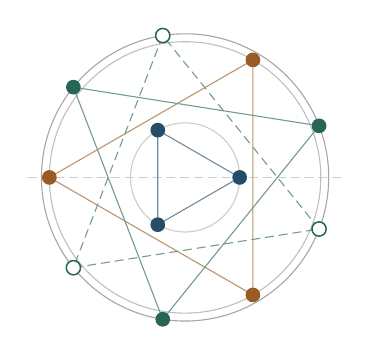
\begin{tikzpicture}[scale=1.66, line cap=round,line join=round]
  \draw[black!20,thin] (0,0) circle (0.417593127);
  \draw[black!25,thin] (0,0) circle (1.038187275);
  \draw[black!35,thin] (0,0) circle (1.098737873);
  \draw[black!20,densely dashed,thin] (-1.20,0)--(1.20,0);
  \draw[inkblue!65,thin] (0:0.417593127)--(120:0.417593127)--(240:0.417593127)--cycle;
  \draw[orbitgold!65,thin] (60:1.038187275)--(180:1.038187275)--(300:1.038187275)--cycle;
  \draw[orbitgreen!65,thin] (21.054593407:1.098737873)--(141.054593407:1.098737873)--(261.054593407:1.098737873)--cycle;
  \draw[orbitgreen!65,thin,densely dashed] (-21.054593407:1.098737873)--(98.945406593:1.098737873)--(218.945406593:1.098737873)--cycle;
  \foreach \a in {0,120,240} \fill[inkblue] (\a:0.417593127) circle[radius=1.6pt];
  \foreach \a in {60,180,300} \fill[orbitgold] (\a:1.038187275) circle[radius=1.6pt];
  \foreach \a in {21.054593407,141.054593407,261.054593407}
    \fill[orbitgreen] (\a:1.098737873) circle[radius=1.6pt];
  \foreach \a in {-21.054593407,98.945406593,218.945406593}
    \draw[orbitgreen,fill=white,line width=.55pt] (\a:1.098737873) circle[radius=1.55pt];
\end{tikzpicture}
\caption{The candidate in the mass-eleven normalization. The solid and dashed green
triangles share the outer circle. The drawing uses rounded coordinates.}
\label{fig:candidate}
\end{figure}

The proof has three finite certificate stages. A rational Ward kernel supplies
a global deficit budget, which becomes a radius restriction through affine
row inequalities. A candidate-saturating kernel is reconstructed from the
exact root and an invertible contact minor. Finally, local and complementary
boxes prove the sharp pointwise inequality. We give the mathematical
implications and the acceptance tests below. The fixed inputs and full replay
programs are available in the \certroot~\cite{archive}.

\section{Stationarity and the kernel summation identity}
\label{sec:ward}

\subsection{Normalization and full stationarity}
Write \(N=\binom{n}{2}\). Multiplying the quadratic mass by \(\eta>0\)
multiplies the optimal product by \(\eta^N\). We use the mass \(n-1\)
normalization throughout the proof, so the multiplier is \(\lambda=n/2\).
A global maximum exists by compactness and has positive product, since
a regular polygon is feasible after scaling. Its points are distinct.
Translating to the centroid preserves the product and reduces the mass
unless the centroid is zero. Rescaling to the prescribed mass would then
strictly increase the product. Thus every global maximizer is centered.

The real Lagrange equations for \(\log\Delta_n\), in complex notation, are
\begin{equation}
 \mathcal F_i(z)=
 \sum_{j\ne i}\frac{1}{z_i-z_j}-\lambda\overline{z_i}=0,
 \qquad \lambda=\frac{N}{Q(z)}.
 \label{eq:stationarity}
\end{equation}
Indeed, multiplying by \(z_i\) and summing counts each unordered pair once.
We also use that a constrained global maximizer at mass \(n-1\) maximizes
\(\Delta_n(z)e^{-\lambda Q(z)}\) on the full configuration space. At a
given positive mass \(q\) the product is bounded by its constrained maximum
at mass \(n-1\) multiplied by \((q/(n-1))^N\). The scalar function
\(q^N e^{-\lambda q}\) is maximized at \(q=n-1\).

\subsection{Positive Gram blocks and zero-sum Ward corrections}
Put \(u=|z|^2\), \(v=|w|^2\), \(t=\RePart(z\bar w)\) and
\(d=u+v-2t\). Set
\[
 H_k(u,v,t)=\RePart((z\bar w)^k),\qquad H_0=1,\quad H_1=t,\quad
 H_k=2tH_{k-1}-uvH_{k-2}\quad(k\ge2).
\]
For real polynomial feature vectors \(f_k\) and real symmetric blocks
\(Q_k\succeq0\) the base kernel
\begin{equation}
 K(u,v,t)=\sum_{k=0}^{11}H_k(u,v,t) f_k(u)^T Q_k f_k(v)
 \label{eq:base-kernel}
\end{equation}
is positive semidefinite. For any real weights on any finite point set
its quadratic form is a sum of squared moment norms. In particular, with
\(U_k=\sum_i z_i^k f_k(|z_i|^2)\) and unit weights,
\begin{equation}
 \sum_{i,j}K_{ij}=\sum_{k=0}^{11}U_k^*Q_k U_k\ge0.
 \label{eq:gram-sum}
\end{equation}

For the corrections use the raw feature vector
\(\phi(u)=(1,u-1,\ldots,(u-1)^4)^T\) and raw moments
\(M_k=\sum_i z_i^k\phi(|z_i|^2)\). These differ from the feature moments
\(U_k\). Let \(p_k=\sum_i z_i^k\), with \(p_0=n\). Multiplication of
\eqref{eq:stationarity} by \(z_i^{k+1}\) and summation give
\begin{equation}
 \lambda\sum_i |z_i|^2z_i^k
 =\left(n-\frac{k+1}{2}\right)p_k+
   \frac12\sum_{r=1}^{k-1}p_rp_{k-r}.
 \label{eq:ward-general}
\end{equation}
For each unordered pair this follows by expanding the difference quotient
\((z_i^{k+1}-z_j^{k+1})/(z_i-z_j)\). Equivalently the right-hand side is
\(\tfrac12\sum_{r=0}^k(p_rp_{k-r}-p_k)\), obtained by subtracting the diagonal
from the ordered sum. For \(n=12\) and \(Q=11\), \(p_1=0\) and the first
two coordinates of \(M_1\) vanish. Moreover \(v_k^T M_k=0\) for \(k=0,2,3\), with
\begin{equation}
 v_0=(1/12,1,0,0,0)^T,\qquad
 v_2=(-3/4,1,0,0,0)^T,\qquad
 v_3=(-2/3,1,0,0,0)^T.
 \label{eq:ward-directions}
\end{equation}
Here \(k=0\) uses the exact mass alone. For \(k=2,3\), the coefficients
follow from \(\sum u_i z_i^2=7p_2/4\) and
\(\sum u_i z_i^3=5p_3/3\).

Choose \(A_1\) real symmetric with zero lower-right \(3\times3\) block and
choose \(A_k=v_k a_k^T+a_kv_k^T\) for \(k=0,2,3\). The first choice has
nine parameters, and each of the others has five. Define
\begin{equation}
 J(u,v,t)=\sum_{k=0}^{3} H_k(u,v,t)\phi(u)^T A_k\phi(v).
 \label{eq:ward-correction}
\end{equation}
Then \(\sum_{i,j}J_{ij}=\sum_{k=0}^3 M_k^* A_k M_k=0\) at every full
stationary configuration of mass eleven. For the rank-two forms this
follows from \(M^*(va^T+av^T)M=2\RePart(\overline{v^T M}\,a^T M)\).
For \(A_1\) it follows from the two zero coordinates. Thus the ordered
sum of \(K+J\) is nonnegative on full stationary configurations, including
every global maximizer.

\subsection{The diagonal correction and the pair deficit}
For any real \(B\) set \(b=(B-66)/12\). Let \(K'=K+J\) and define
\begin{equation}
 P_B(u)=\frac{6u+b-\tfrac12 K'(u,u,u)}{11},\qquad
 h(u,v,t)=P_B(u)+P_B(v)-K'(u,v,t).
 \label{eq:pair-h}
\end{equation}
Each \(P_B(u_i)\) appears eleven times in the unordered pair sum.
Consequently, at mass eleven,
\begin{equation}
 \sum_{i<j}h_{ij}
 =B-\frac12\sum_{i,j}K'_{ij}
 =B-\frac12\sum_{i,j}K_{ij}
 \quad\text{at full stationary configurations}.
 \label{eq:kernel-sum}
\end{equation}
The first equality uses the mass alone. The second uses the Ward
identities. When \(h+\varepsilon\ge\log d\) on a necessary pair domain,
the nonnegative pair deficits and the Gram penalties satisfy the exact
budget identity
\begin{equation}
 \sum_{i<j}(h_{ij}+\varepsilon-\log d_{ij})
 +\frac12\sum_{k=0}^{11}U_k^*Q_kU_k
 =B+66\varepsilon-\log\Delta_{12}(z).
 \label{eq:budget}
\end{equation}
We first apply \eqref{eq:budget} with a small positive \(\varepsilon\)
to localize every maximizer. The final application takes
\(B=\log\Delta_{12}(z^*)\) and \(\varepsilon=0\).

\section{The necessary pair domain and the radial population}
\label{sec:radial-domain}

Throughout this section \(x\) is a global maximizer at mass eleven and
\(\Delta=\Delta_{12}(x)\). We use its centering and full stationarity from
Section~\ref{sec:ward}.

\subsection{Strict subset bounds}

Use the unconstrained objective \(\Delta(x)e^{-6Q(x)}\) from
Section~\ref{sec:ward}. Fix a proper subset \(S\) of size
\(m\ge2\), with centroid \(a\), centered points \(y_i=x_i-a\), and mass
\(q=\sum_{i\in S}|y_i|^2\). Replacing its points by \(a+\zeta y_i\) leaves
the part of the objective depending on \(\zeta\) proportional to
\[
 |\zeta^k P(\zeta)|^2e^{-6q|\zeta|^2},\qquad
 k=\frac{m(m-1)}2,\qquad
 P(\zeta)=\prod_{i\in S,\,j\notin S}(a+\zeta y_i-x_j).
\]
The point \(\zeta=1\) maximizes this expression. Thus \(f=P/P(1)\) satisfies
\(f(1)=1\) and \(|f|\le1\) on the unit disk. Differentiation in the radial
and angular directions at \(1\) gives \(f'(1)=\delta=6q-k\). Also
\(P'(0)=0\), since the coefficient of \(\zeta\) in the product for each
fixed \(j\notin S\) is a multiple of \(\sum_{i\in S}y_i\).

The polynomial \(P\) is nonconstant, since the factors are nonzero
polynomials and at least one has nonzero slope. Put \(A=f(0)\), so
\(|A|<1\). The disk map \(g=(f-A)/(1-\overline A f)\) vanishes to order
at least two at zero. The Schwarz lemma gives \(g(\zeta)=\zeta^2 j(\zeta)\)
with \(|j|\le1\). Because \(|j(1)|=1\), the inward radial limit implies
\(\RePart(j'(1)/j(1))\ge0\). Consequently,
\begin{equation}
 \delta\ge 2\frac{|1-A|^2}{1-|A|^2}
 \ge 2\frac{1-|A|}{1+|A|}>0.
 \label{eq:domain-schwarz}
\end{equation}
The strict subset bound is \(q>m(m-1)/12\). For \(0<\delta<2\),
\eqref{eq:domain-schwarz} also gives
\begin{equation}
 |P(1)|^2\le S(\delta)|P(0)|^2,\qquad
 S(\delta)=\left(\frac{2+\delta}{2-\delta}\right)^2.
 \label{eq:domain-cross-factor}
\end{equation}

For two selected points \(z,w\), set
\(u=|z|^2\), \(v=|w|^2\), \(t=\RePart(z\overline w)\), and \(d=u+v-2t\).
The subset consisting of these two points has mass \(d/2>1/6\).
Deleting the point \(z\) leaves an eleven-point subset of mass
\(11-12u/11>55/6\). Together with the Gram inequality these give the
closed preliminary domain
\begin{equation}
 \mathcal D_0=\{(u,v,t):0\le u,v\le U_0,\ t^2\le uv,\ d\ge1/3\},
 \qquad U_0=121/72.
 \label{eq:domain-preliminary}
\end{equation}
The radius and separation inequalities are strict at every maximizer.

\subsection{One- and two-point deletion}

The finite disk-smearing bound for \(m\) points with centered mass \(q\)
is
\[
 U_m(q)=m^{m/2}\left(\frac{2q}{m-1}\right)^{m(m-1)/2}
 e^{-m(m-1)/4}.
\]
At mass \(m-1\), write \(g(x)=-\log|x|\) and let
\(D(\nu)=\iint g(x-y)\,d\nu(x)\,d\nu(y)\). The functional
\(D(\nu)+\tfrac12\int |x|^2\,d\nu\) is minimized among compactly supported
probabilities of bounded density by the uniform disk \(\nu_0\) of radius
\(\sqrt2\), with value \(3/4-\tfrac12\log2\). The logarithmic potential
\(g*\sigma_R\) of a uniform disk of radius \(R\) is
\(-\log R+1/2-|x|^2/(2R^2)\) inside and \(-\log|x|\) outside. With
\(R=\sqrt2\), the sum \(g*\nu_0+|x|^2/4\) is constant on the disk and
at least this constant outside. For \(\eta=\nu-\nu_0\), the quadratic
term in the energy comparison is
\(D(\eta)=(2\pi)^{-1}\int|\nabla(g*\eta)|^2\ge0\), by integration by
parts using the zero total mass of \(\eta\). Integrating the disk
potential and the confinement term gives the stated minimum.

Replace each point by a uniform disk of radius \(r\), and let \(\nu\)
be the average of these disk measures. The average of \(g\) over
translations by one disk is at most \(g\), and the same is true for
two disks. The self-energy of one disk is \(-\log r+1/4\), and
\(\int |x|^2\,d\nu=(m-1)/m+r^2/2\). Subtracting the \(m\) self-terms
from \(m^2D(\nu)\) thus gives
\[
 -\log\Delta_m\ge m^2(3/4-\tfrac12\log2)
 -\frac{m(m-1)}2-\frac{m^2r^2}4+m\log r-\frac m4.
\]
Set \(r^2=2/m\) and scale from mass \(m-1\) to \(q\) to obtain
\(U_m(q)\). This is the finite argument in
\texttt{asymptotics/proof.tex} of the accompanying repository. It
applies to each remaining subset without a stationarity hypothesis.
Define rational upper constants by
\[
 E(x)=\sum_{j=0}^{100}\frac{x^j}{j!},\qquad
 C_{11}=\frac{11^5(33166248/10^7)(1/5)^{55}}{E(55/2)},\qquad
 C_{10}=\frac{10^5(2/9)^{45}}{E(45/2)}.
\]
The positive exponential series and \((33166248/10^7)^2>11\) give
\(U_{11}(q)<C_{11}q^{55}\) and \(U_{10}(q)<C_{10}q^{45}\) for \(q>0\).
Let \(V^{(11)}\) be the value of the fixed integer witness in mass eleven.
For its original integer points \(b_i\), this is \((132/D)^{66}P_0\),
where \(D=12\sum_i|b_i|^2-|\sum_i b_i|^2\) and
\(P_0=\prod_{i<j}|b_i-b_j|^2\). The \(b_i\) are the twelve Gaussian
integers in the \(n=12\) entry of the fixed archive's
\texttt{symmetry-breaking/integer\_witnesses.json}.

After one deletion, the interaction constant in
\eqref{eq:domain-cross-factor} is \(|P(0)|^2=(144u/121)^{11}\).
For \(81/50\le u<121/72\) we have \(0<\delta=6q-55<2\), and hence
\[
 \Delta\le F_{11}(u)=C_{11}q^{55}(144u/121)^{11}S(\delta),
 \qquad q=11-12u/11.
\]
The logarithmic derivative of \(F_{11}\) is strictly below
\(11/u-144/11<0\), using \(q'<0\) and
\((2+\delta)^{-1}+(2-\delta)^{-1}\ge1\). Exact rational evaluation gives
\(F_{11}(81/50)<(997/1000)V^{(11)}\). Thus every maximizer has
\begin{equation}
 u<81/50.
 \label{eq:domain-deletion-radius}
\end{equation}

For two deletions let \(a=-(z+w)/10\) be the remaining centroid. Now
\[
 \begin{aligned}
 q&=11-\frac{11(u+v)+2t}{10},\qquad \delta=6q-45,\\
 b&=|z-a|^2|w-a|^2=\frac{(121u+v+22t)(u+121v+22t)}{10^4}.
 \end{aligned}
\]
The ten-point subset has \(q>15/2\). When \(\delta<2\), its interaction
constant is \(b^{10}\), and the two deleted points contribute \(d\).
This gives the necessary rational inequality
\begin{equation}
 (2+\delta)^2 C_{10}q^{45}d\,b^{10}
 \ge (2-\delta)^2 V^{(11)}.
 \label{eq:domain-pair-deletion}
\end{equation}
For \(R=11-q\) and \(s=d/2\), the centroid decomposition gives
\(0\le s\le R\) and \(|z-a|^2+|w-a|^2=(6R-s)/5\). Thus
\[
 d\,b^{10}\le 2s\left(\frac{6R-s}{10}\right)^{20}
 \le (4R/7)^{21}.
\]
The last upper bound occurs at \(s=2R/7\), as the derivative of
\(s(6R-s)^{20}\) is \((6R-s)^{19}(6R-21s)\). On
\(15/2<q\le7573/1000\), the resulting upper bound
\(F_{10}(q)=C_{10}q^{45}(4(11-q)/7)^{21}S(6q-45)\) is increasing, since
its logarithmic derivative is at least \(45/q-21/(11-q)+12>0\).
Exact arithmetic gives \(F_{10}(7573/1000)<(992/1000)V^{(11)}\), so
\(q>7573/1000\), or equivalently \(11(u+v)+2t<3427/100\).
Equations \eqref{eq:domain-preliminary}, \eqref{eq:domain-deletion-radius},
and \eqref{eq:domain-pair-deletion}, with this last linear bound, give
analytic necessary pair restrictions. The one-deletion radius bound
will be used for the upper tail of the row cuts. The two-deletion
inequalities supply an additional pruning test. The endpoint and witness
computations are replayed by \texttt{twelve-point-removal-domain/}\allowbreak
\texttt{verify\_all.py}.

\subsection{Ward deficit and the two radial bands}

\begin{lemma}[Preliminary rational majorant]\label{lem:preliminary}
The fixed rational kernel \(K_{\mathrm W}\) has twelve positive definite
base Gram blocks. Its correction has the Ward form
\eqref{eq:ward-correction}. With
\[
 B_{\mathrm W}=\frac{7726135064073933}{281474976710656},
 \qquad c_0=\frac1{25000},
\]
its pair function satisfies \(h_{\mathrm W}+c_0\ge\log d\) throughout
\(\mathcal D_0\).
\end{lemma}

The replay reads \texttt{twelve-point-ward-upper/}\allowbreak\texttt{kernel.json}
and tests every base block by exact rational \(LDL^T\)
factorization and constructs the raw Ward blocks from their 24 rational
parameters. It checks 57 bilinear restrictions on the relevant moment
subspaces and reconstructs the polynomial of multidegree at most
\((19,19,11)\). In the root box \([0,U_0]^2\times[-U_0,U_0]\) it converts
this polynomial to tensor Bernstein coefficients. Every midpoint
subdivision rounds its lower coefficients down. Each leaf is accepted
by a rational upper tangent to \(\log d\), with \(c_0\) added to
\(h_{\mathrm W}\), or by exclusion from the physical domain or the
ordered half \(u\le v\). Symmetry covers the other half. This uses the
same bounding principle described in Section~\ref{sec:cover}. The
archived replay accepts all 268,239 nodes, including 127,832 inequality
leaves and 6,288 discarded leaves.

Let \(G=h_{\mathrm W}+c_0-\log d\) and let \(K_{\mathrm W}\) denote the
base kernel. At a
global maximizer, the Ward corrections sum to zero over ordered pairs.
The diagonal-corrected summation identity therefore gives
\begin{equation}
 \sum_{i<j}G_{ij}+\frac12\sum_{i,j}K_{\mathrm W}(x_i,x_j)
 =B_{\mathrm W}+66c_0-\log\Delta
 <66c_0.
 \label{eq:domain-deficit}
\end{equation}
Here \(\Delta\ge V^{(11)}\). A positive-term logarithm expansion after
dyadic range reduction gives a rational lower bound for \(\log V^{(11)}\)
strictly above \(B_{\mathrm W}\). The pair terms and the ordered sum of
each positive Gram block are nonnegative.

For a marked point of radius squared \(u\), its eleven neighbors satisfy
\(\sum_{j\ne i}v_j=11-u\) and \(\sum_{j\ne i}t_j=-u\). The certificate
partitions \([0,3/25]\), \([6/25,47/50]\), and \([71/50,33/20]\) into
53 closed subintervals with adjacent endpoints. For each subinterval
\(J\), fixed rational coefficients \(a_J,b_J\) satisfy the continuous
inequality
\begin{equation}
 G(u,v,t)\ge\frac1{4000}
 +a_J\left(v-\frac{11-u}{11}\right)+b_J\left(t+\frac u{11}\right)
 \quad\bigl((u,v,t)\in\mathcal D_0,\ u\in J\bigr).
 \label{eq:domain-row-cut}
\end{equation}
The verifier subtracts the two affine terms from the rational polynomial
\(h_{\mathrm W}\). On each accepted box the Bernstein coefficients,
rounded down under midpoint subdivision, dominate an upward enclosure of
\(\log\xi+(d-\xi)/\xi-c_0+1/4000\) for a positive rational \(\xi\).
Concavity makes this an upper bound for \(\log d-c_0+1/4000\).
Pruned boxes violate
the Gram or separation condition. The roles of \(u\) and \(v\) stay
fixed because \(u\) marks the row. The 53 trees contain 99,603 nodes,
including 46,539 inequality leaves and 3,289 discarded leaves, with
every partition closed.

Summing \eqref{eq:domain-row-cut} over the neighbors cancels the affine
terms, leaving \(11/4000>66c_0\), in contradiction to
\eqref{eq:domain-deficit}. The upper tail is excluded by
\eqref{eq:domain-deletion-radius} since \(81/50<33/20\). Every squared
radius therefore lies in one of the open bands
\[
 I=(3/25,6/25),\qquad O=(47/50,71/50).
\]

\subsection{The inner population is three}

Let \(Q_0\) be the radial Gram block of \(K_{\mathrm W}\), and let
\(m=\sum_i F_0(u_i)\) be its radial moment vector. Its first four
coordinates are \(\sum_i(u_i^j-\mu_j)\), \(1\le j\le4\), with the
rational centers \(\mu_j\) read from the fixed kernel. The radial part
of \eqref{eq:domain-deficit} gives \(m^TQ_0m<132c_0\). Delete the first
row and column of \(Q_0\) to obtain \(Q_0^{\mathrm{tail}}\), solve
\(Q_0^{\mathrm{tail}}y=(-4,1,0,0)^T\), and put \(w=(0,y)^T\).
Exact substitution verifies the solution and \(w^TQ_0w<20\). Set
\(p(u)=u^3-4u^2+4\mu_2-\mu_3\). The difference between \(w^TQ_0m\)
and \(\sum_i p(u_i)\) is \((11-12\mu_1)(Q_0w)_1\), whose absolute
value is strictly below \(1/10000\) by rational computation. Thus
\[
 \left|\sum_i p(u_i)\right|
 <\frac1{10000}+\sqrt{20\cdot132c_0}<\frac{41}{100}.
\]

The following lower bounds are verified by nonnegative cubic Bernstein
coefficients on 64 equal subintervals of each indicated band, for each
sign.
\[
\begin{array}{c|cc}
 &u\in\overline I &u\in\overline O\\ \hline
 p(u) & 347/100-(26/5)u & 509/100-(26/5)u\\
 -p(u) & -199/50+(531/100)u & -263/50+(531/100)u
\end{array}
\]
If the inner population is \(k\le2\), the first row and \(\sum_i u_i=11\)
give \(\sum_i p(u_i)\ge(388-162k)/100\ge16/25\). If \(k\ge4\), the
second row gives \(-\sum_i p(u_i)\ge(128k-471)/100\ge41/100\).
Both contradict the radial bound. Hence every global maximizer has
exactly three points in \(I\) and nine in \(O\). The row and population
checks are replayed by \texttt{twelve-point-ward-radii/}\allowbreak\texttt{verify\_all.py}.
The subsequent pair comparison can therefore use the closures of the
three radial products \(I\times I\), \(I\times O\), and \(O\times O\),
intersected with the Gram and separation conditions.

\section{The twelve-point candidate}
\label{sec:candidate}

We use the mass-$11$ normalization of Section~\ref{sec:ward}. The candidate is specified by an isolating box for the full force equations. The original box is in mass $12$, where the multiplier is $11/2$. In real coordinates the force at the $i$th point is
\[
 \mathcal F_i(y)=\sum_{j\ne i}\frac{y_i-y_j}{|y_i-y_j|^2}
                   -\frac{11}{2}y_i.
\]
Fix the rotational gauge $\operatorname{Im}y_0=0$, $\operatorname{Re}y_0>0$, and omit the imaginary component of the force at $y_0$. Let $f$ denote the resulting map on $23$ real variables. The certificate specifies a dyadic center $m$, a closed sup-norm box $X$ of radius $r=2^{-80}$, and a dyadic preconditioner $C$. Outward integer interval evaluation verifies that the box is collision free, that the real part of its first point is positive, and that
\[
 \|Cf(m)\|_\infty\le 2^{-257},\qquad
 \sup_{x\in X}\|I-CDf(x)\|_\infty\le 2^{-66}.
\]
The map $x\mapsto x-Cf(x)$ is a contraction from $X$ into itself. The derivative bound makes $CDf(x)$, hence $C$, invertible, so its unique fixed point is the unique zero of $f$ in the box. The a posteriori bound $\|Cf(m)\|_\infty/(1-2^{-66})$ encloses this zero within $2^{-256}$ of $m$. These data and checks are in \texttt{validated-maxima/}\allowbreak\texttt{certificates.json} and \texttt{validated-maxima/}\allowbreak\texttt{verify\_all.py} at repository revision \texttt{3c922f3}.

The identity $\sum_i\operatorname{Im}(\overline y_i\mathcal F_i)=0$ follows by grouping the two forces of each pair. It recovers the omitted equation because $y_0$ is positive real. Summing the full equations gives centering. Taking their real scalar product with the coordinates gives $(11/2)\sum_i |y_i|^2=66$. Clearing denominators in the collision-free rational isolating box specifies a unique real solution of a rational polynomial system there, so its coordinates are real algebraic.

The symmetry check uses the smaller a posteriori enclosure. A saved permutation of order three is followed by regauging its first point to the positive real axis. A second saved permutation is treated in the same way after conjugation. The two transformed roots satisfy the force equations and lie in the original uniqueness box. The interval bounds put both transformed roots within $2^{-254}$ of its center. Uniqueness identifies them with the original root. The permutations generate a dihedral group of order six. The resulting point orbits have sizes $3,3,6$ and their squared-radius intervals are disjoint. The symmetry permutations and their replay are recorded in \texttt{candidate-global-screen/}.

Rescale by $\sqrt{11/12}$, and rotate a point of the innermost triangle to the positive real axis. Write $\omega=e^{2\pi i/3}$. The exact candidate $z^*$ is the union of the four orbits
\begin{equation}
 \{a\omega^j\}_{j=0}^2,\qquad
 \{-b\omega^j\}_{j=0}^2,\qquad
 \{(c+i d_0)\omega^j\}_{j=0}^2,\qquad
 \{(c-i d_0)\omega^j\}_{j=0}^2,
 \label{eq:n12-candidate-shape}
\end{equation}
with $a,b,c,d_0>0$. The certified reflection fixing the inner point gives the real axis in this gauge. Its fixed point on the middle triangle is negative real, and the outer orbit has a representative with both coordinates positive. These signs are checked on the root enclosure. In particular, $a^2\in(17/100,18/100)$ and $b^2\in(107/100,109/100)$. The orbits of unordered pairs give fourteen distinct triples $(u,v,t)$ after ordering the radii. Thirteen satisfy $t^2<uv$. The remaining triple comes from the opposite inner and middle rays and has $t=-\sqrt{uv}$. The orbit multiplicities sum to $66$. The squared radii in mass
eleven are approximately \(0.17438402\), \(1.07783282\), and \(1.20722491\).
Table~\ref{tab:contacts} lists the contact orbits in certificate order.

\begin{table}[tb]
\centering
\small
\setlength{\tabcolsep}{4pt}
\begin{tabular}{@{}rccrr@{\quad}rccrr@{}}
\toprule
No. & Layers & \(t\) & Mult. & \(r\) &
No. & Layers & \(t\) & Mult. & \(r\)\\
\midrule
1  & \(3,3\) & \( 0.25324601\) & 3 & \(2^{-8}\) &
8  & \(2,2\) & \(-0.53891641\) & 3 & \(2^{-7}\)\\
2  & \(3,3\) & \(-0.60361246\) & 6 & \(2^{-8}\) &
9  & \(1,3\) & \(-0.07134427\) & 6 & \(2^{-9}\)\\
3  & \(3,3\) & \( 0.89560194\) & 3 & \(2^{-10}\) &
10 & \(1,3\) & \( 0.42819353\) & 6 & \(2^{-8}\)\\
4  & \(2,3\) & \(-1.06454117\) & 6 & \(2^{-9}\) &
11 & \(1,2\) & \( 0.21676994\) & 6 & \(2^{-8}\)\\
5  & \(2,3\) & \( 0.17737052\) & 6 & \(2^{-8}\) &
12 & \(1,3\) & \(-0.35684926\) & 6 & \(2^{-8}\)\\
6  & \(2,3\) & \( 0.88717064\) & 6 & \(2^{-10}\) &
13 & \(1,2\) & \(-0.43353987\) & 3 & \(2^{-11}\)\\
7  & \(3,3\) & \(-1.14884795\) & 3 & \(2^{-11}\) &
14 & \(1,1\) & \(-0.08719201\) & 3 & \(2^{-7}\)\\
\bottomrule
\end{tabular}
\caption{The fourteen unordered pair orbits. Layers are numbered outward,
\(t\) is rounded for display, and \(r\) is the nominal local-box radius used
in Section~\ref{sec:cover}. Orbit 13 is on the Gram boundary.}
\label{tab:contacts}
\end{table}

For later use, the certificate also encloses the third moment of each radius layer in the axis gauge. The two triangle moments have the moduli dictated by their radii. On the outer layer, with squared radius $s_3=c^2+d_0^2$, it verifies
\[
 0<\left|\sum_{|z_i^*|^2=s_3}(z_i^*)^3\right|<6s_3^{3/2}.
\]
The interval computation can use $(z_i^*\overline w)^3$ for an inner axis point $w$, and compare squared moduli before dividing out the common factor $|w|^6$. This test separates the outer third moment from zero and from the endpoint where the two cubed representatives coincide. The layer tests are in \texttt{candidate-global-screen/symmetry\_report.json}.

If $w_1,\ldots,w_4$ are the cubes of the four representatives in \eqref{eq:n12-candidate-shape}, the candidate value in mass $12$ is
\begin{equation}
 C_{12}=\left(\frac{12}{11}\right)^{66}
 27^4\prod_{i=1}^4|w_i|^2\prod_{i<j}|w_i-w_j|^6.
 \label{eq:n12-candidate-value}
\end{equation}
The factor $z^3-w_i$ contributes $27|w_i|^2$ within its triangle. The squared modulus of the resultant of $z^3-w_i$ and $z^3-w_j$ gives $|w_i-w_j|^6$ between triangles.

\section{Exact contact interpolation}
\label{sec:contacts}

Set $B=\log\Delta(z^*)$ in mass $11$ and use the diagonal correction of Section~\ref{sec:ward}. Put $u_i^*=|z_i^*|^2$ and denote the three distinct squared radii by $s_1,s_2,s_3$. Define
\[
 \mu_j=\frac1{12}\sum_i(u_i^*)^j,\qquad
 q(u)=\prod_{r=1}^3(u-s_r),\qquad
 F_0(u)=(u-\mu_1,u^2-\mu_2,u^3-\mu_3,u^4-\mu_4,10q(u)^2)^T.
\]
The radial feature sum at the candidate is zero. For the other blocks use $\phi_j(u)=(u-1)^j$, $0\le j\le4$, and write $M_k^*=\sum_i(z_i^*)^k\phi(u_i^*)$ for the raw moment vector. For $1\le k\le11$ with $3\nmid k$, use the five raw features. Their candidate moments vanish by the rotation of order three. For $k=3,6,9$, use the four features
\[
 \phi_j(u)-\frac{(M_k^*)_j}{(M_k^*)_0},\qquad 1\le j\le4.
\]
The ratios are real by reflection in the chosen axis. The root interval verifies all three denominators are nonzero. Each adapted feature sum is therefore zero in its harmonic. There are nine symmetric Gram blocks of size five and three of size four, giving $165$ independent Gram entries. The ordered-pair sum of the base kernel and its first differential vanish at $z^*$ for every choice of these entries.

\subsection{First-order restrictions on the Ward correction}

Use the Ward blocks of Section~\ref{sec:ward}, with the vector parameter in $A_k=v_k a_k^T+a_k v_k^T$ denoted by $a_k$. For $k=0,3$ impose
\begin{equation}
 a_0^TM_0^*=a_3^TM_3^*=0.
 \label{eq:n12-contact-ward-null}
\end{equation}
Together with $v_k^TM_k^*=0$, these conditions give $A_kM_k^*=0$. The corresponding products for $k=1,2$ vanish because $M_1^*=M_2^*=0$. Thus the Ward ordered-pair sum also has zero first differential at the candidate. Each condition in \eqref{eq:n12-contact-ward-null} eliminates the constant coordinate of its vector parameter. With nine parameters in $A_1$, five in $A_2$, and four in each of $A_0,A_3$, the Ward correction has $22$ parameters.

These two eliminations can also be read directly from sharp contact. All candidate pairs are strict in the radius and distance bounds. Small variations of the actual points preserve the Gram condition, including at the collinear pair. If $G=h-\log d$ is nonnegative there and vanishes at every candidate pair, the sum of its values has zero first differential. Along the dihedral family \eqref{eq:n12-candidate-shape}, the differential of that sum is
\[
 -(a_0^TM_0^*)\,\mathrm dQ-(a_3^TM_3^*)\,\mathrm dW_3,
 \qquad W_3=\sum_i (|z_i|^2-5/3)z_i^3.
\]
Indeed $v_0^TM_0=Q-11$, $v_3^TM_3=W_3$ is real in this family, and the force equations give $\mathrm d\log\Delta=6\,\mathrm dQ$ at the candidate. The variation $\dot a=b$, $\dot b=-a$, $\dot c=\dot d_0=0$ has $\mathrm dQ=0$ and
\[
 \mathrm dW_3=15ab\bigl[a(a^2-1)+b(b^2-1)\bigr]<0.
\]
The sign follows from the two certified radius intervals. This variation forces $a_3^TM_3^*=0$. A variation with nonzero $\mathrm dQ$ then forces $a_0^TM_0^*=0$.

\subsection{The five compatibility relations}

Let $\theta\in\mathbb R^{187}$ contain the Gram and Ward entries. Write
\[
 h=h_0+\mathcal H_\theta,
 \qquad h_0=\frac6{11}(u+v)+\frac{B-66}{66},
\]
so that $\mathcal H_\theta$ is linear in $\theta$. At each contact impose the value condition $G=0$. At the thirteen interior contacts impose $\nabla G=0$. At the boundary contact impose the two derivatives of $G(u,v,-\sqrt{uv})$ to be zero. These are $G_u+tG_t/(2u)=0$ and $G_v+tG_t/(2v)=0$. Six interior contacts have $u=v$, where exchange symmetry identifies $G_u$ and $G_v$. After dropping these duplicates there are $14$ value rows and $35$ derivative rows. Write the resulting system as $L\theta=y$, where $y$ contains the corresponding values and derivatives of $\log d-h_0$.

For explicit matrix construction, let $K'_\theta$ be the sum of the base kernel and its Ward correction. The column for a parameter is obtained by evaluating and differentiating its contribution to
\[
 \mathcal H_\theta(u,v,t)=-K'_\theta(u,v,t)
 -\frac{K'_\theta(u,u,u)+K'_\theta(v,v,v)}{22}.
\]
In particular the derivatives of the two diagonal terms enter the radial rows. At each contact the derivative of $\log d$ is $(1,1,-2)/d$, so only the value rows require logarithms on the right-hand side. The entries of $L$ are algebraic.

One row relation is the sum of the value rows with the pair-orbit multiplicities as weights. It vanishes on $\mathcal H_\theta$ because the candidate kernel sum is zero. It also vanishes on the right-hand side, since the weighted sum of $\log d$ is $B$ and that of $h_0$ is $B$.

Four more relations come from varying $a,b,c,d_0$ in \eqref{eq:n12-candidate-shape}. In each direction apply the chain rule to the multiplicity-weighted sum over the contacts. The derivative of the kernel sum is zero by the adapted features and \eqref{eq:n12-contact-ward-null}. On the right-hand side, both $\log\Delta$ and the sum of $h_0$ have differential $6\,\mathrm dQ$. On the boundary orbit, the variation stays on $t=-\sqrt{uv}$, so the chain rule uses the two retained tangent rows. On an equal-radius orbit it uses the retained radial row with the sum of the two radial velocities.

The four derivative relations are independent. A variation giving the zero row combination has zero contact velocities in all the retained coordinates, since each orbit multiplicity is positive. In particular it has zero differentials of $a^2$, $b^2$, $c^2+d_0^2$, and the inner--outer dot product $ac$. These four differentials are independent because $a,b,d_0$ are positive. The value relation is supported on different rows. Hence the five relations are independent and $\operatorname{rank} L\le44$.

\subsection{Certified rank and correction of the seed}

The stored row and column sets $I,J$ specify a $44\times44$ minor. Rebuilding its entries from the isolated root and applying outward interval Gaussian elimination on the $2^{-384}$ lattice verifies that every pivot excludes zero and that the determinant interval excludes zero. Thus $\operatorname{rank}L=44$, and the five analytic identities give all row compatibility conditions. The row and column sets are recorded in \texttt{twelve-point-sharp-contacts/}\allowbreak\texttt{minor.json}.

The global certificate takes the dyadic Gram and Ward seed from \texttt{twelve-point-banded-upper/}\allowbreak\texttt{kernel.json}. Each harmonic Gram block is transferred through its stored change-of-basis matrix. For $k=3,6,9$ the transfer uses the last four rows, since the constant coefficient of each adapted feature is supplied by the exact candidate moment ratio. The radial features use the exact nodes and means, and the constant coordinates of $a_0,a_3$ are supplied by \eqref{eq:n12-contact-ward-null}. Denote the resulting seed in the $187$ coordinates by $\theta^{(0)}$. The exact corrected coefficients are defined by
\begin{equation}
 \theta_J=\theta^{(0)}_J+L_{IJ}^{-1}
       \bigl(y_I-(L\theta^{(0)})_I\bigr),\qquad
 \theta_{J^c}=\theta^{(0)}_{J^c}.
 \label{eq:n12-contact-correction}
\end{equation}
The selected equations hold by construction. The row relations extend them to all $49$ equations, because $y$ satisfies those relations. This specifies the coefficients as exact real expressions in the algebraic candidate data and the contact logarithms.

For interval evaluation, each contact distance is scaled by a power of two into $[1,2]$. With $r=(s-1)/(s+1)$ for the scaled distance $s$, the logarithm enclosure uses $2\sum_{j=0}^{99}r^{2j+1}/(2j+1)$ and the remainder bound $2r^{201}/(201(1-r^2))$. The same series encloses $\log2$. The replay encloses the solve in \eqref{eq:n12-contact-correction}, checks all contact residual intervals, and applies interval $LDL^T$ factorization to the twelve corrected Gram blocks. Every Gram block is strictly positive definite, with all pivots greater than $2^{-17}$. It also certifies positive Hessians at the thirteen interior contacts and for the restriction to the Gram face at the boundary contact, with $-tG_t>2^{-13}$ there. The reconstruction is implemented in \texttt{twelve-point-sharp-global/}\allowbreak\texttt{kernel\_bridge.py} and recorded in its verification report.

\section{Zero-slack coverage of the pair domain}
\label{sec:cover}

Work at mass \(11\), and let \(z^*\) denote the isolated candidate.
Use the function \(h\) from Section~\ref{sec:ward}, with the coefficients
reconstructed in Section~\ref{sec:contacts} and with
\(B=\log\Delta(z^*)\). Write
\[
 d=u+v-2t,\qquad G(u,v,t)=h(u,v,t)-\log d.
\]
By Section~\ref{sec:radial-domain}, every pair in a global maximizer has
its squared radii in the two bands
\(I=(3/25,6/25)\) and \(O=(47/50,71/50)\).
We use their closures in the cover. Since \(h\) and \(d\) are symmetric
in \(u,v\), we order the radii by \(u\le v\). The remaining constraints
are \(t^2\le uv\) and \(d\ge 1/3\). The three radial rectangles are
\(\overline I^2\), \(\overline I\times\overline O\), and
\(\overline O^2\). For these rectangles take, respectively,
\(R=6/25,3/5,71/50\), so that \(\sqrt{uv}\le R\). Appending the
intervals \([-R,0]\) and \([0,R]\) gives six rational root boxes.

\subsection{The fourteen contact neighborhoods}

For an exact contact \(p_*=(u_*,v_*,t_*)\), put \(d_*=u_*+v_*-2t_*\)
and \(s=(d-d_*)/d_*\). The polynomial
\begin{equation}
 P_*(p)=h(p)-\log d_*-\left(s-\frac{s^2}{2}+\frac{s^3}{3}\right)
 \label{eq:n12-cover-cubic}
\end{equation}
is a lower bound for \(G\) wherever \(d>0\). Indeed, the derivative of
\(s-s^2/2+s^3/3-\log(1+s)\) is \(s^3/(1+s)\). The difference therefore
has its minimum zero at \(s=0\) on \(s>-1\). In coordinates translated
by \(p_*\), the constant coefficient of \(P_*\) is exactly zero by
the contact equation. The linear term agrees with that of \(G\).
The checker inserts the exact zero constant and encloses the other
translated coefficients by outward rounding on the \(2^{-384}\)
dyadic grid.

For each of the thirteen interior contacts, the local data supply a
dyadic radius \(r\) and a dyadic \(3\times3\) congruence matrix \(W\).
On the full cube of offsets \([-r,r]^3\), the checker bounds the
polynomial entries of \(W^T\nabla^2P_*W\) and verifies positivity
by interval \(LDL^T\) elimination. The resulting positive definite
congruence implies that \(W\) is invertible and that \(\nabla^2P_*\)
is positive definite throughout the cube. The cube lies in \(d>0\).
Since \(P_*(p_*)=0\) and \(\nabla P_*(p_*)=0\), integration of the
second derivative along the segment from \(p_*\) to \(p\) yields
\(P_*(p)\ge0\), with equality only at \(p_*\).

The remaining contact is antiparallel and lies on the Gram face
\(t=f(u,v)=-\sqrt{uv}\). Here the proof box has half-widths
\((r,r,2r)\). The checker verifies \(u,v,d>0\) on this box, verifies
that the projection \(\psi(u,v)=(u,v,f(u,v))\) lies in it for every
base point, and proves \(\partial_tP_*>0\) throughout the box.
On the face it bounds the two-dimensional Hessian
\[
 \nabla^2(P_*\circ\psi)
   =D\psi^T(\nabla^2P_*)D\psi
       +(\partial_tP_*)\nabla^2f.
\]
The last row of \(D\psi\) is \((f/(2u),f/(2v))\). The diagonal
entries of \(\nabla^2f\) are \(-f/(4u^2)\) and \(-f/(4v^2)\),
and the off-diagonal entry is \(f/(4uv)\). Interval \(LDL^T\)
verifies positive definiteness over the full base rectangle.
The exact tangential contact equations make \(p_*\) the unique
minimum on this projected rectangle. Every feasible point in the
proof box satisfies \(t\ge f(u,v)\), and the vertical segment from
the face to that point lies in the box. Positivity of
\(\partial_tP_*\) thus extends \(P_*\ge0\) from the face to the
feasible side. Equality again occurs only at the contact.

The replay verifies all fourteen local boxes. Their smallest
nominal radius is \(2^{-11}\), and the lower bound \(2^{-9}\)
applies to the pivots in the verified local congruences and the
boundary restriction. To assign a rational cover leaf to a
contact, the checker uses a rational box contained in the
certified box about the exact center. Specifically, if a center
coordinate is enclosed by \([L,U]\), it uses \([U-r,L+r]\)
in that coordinate, and checks that this interval has positive
length. This is the intersection of the radius-\(r\) intervals
over all centers in \([L,U]\). The same nominal \(r\) is used
for the boundary contact's rational assignment box.

\subsection{The signed Bernstein cover}

Write \(h=\sum c_{ijk}u^iv^jt^k\), with the real coefficients
enclosed by rational intervals. On each signed root box we
construct a rational polynomial lower envelope for \(h\). For
a nonnegative monomial we use the lower coefficient endpoint.
For an odd power of \(t\) on the nonpositive half, we use the
upper endpoint. The signs are fixed because \(u,v\ge0\).
This produces a pointwise lower envelope on the whole root box.

The envelope is converted to the tensor Bernstein basis of
degrees \((19,19,11)\). To describe the conversion, first map
the box affinely to the unit cube. If \(\widetilde c_\alpha\)
are the resulting power coefficients and \(m=(19,19,11)\),
the control coefficient at multi-index \(r\) is
\[
 \beta_r=\sum_{\alpha\le r}\widetilde c_\alpha
           \prod_{\ell=1}^3
           \frac{\binom{r_\ell}{\alpha_\ell}}
                {\binom{m_\ell}{\alpha_\ell}}.
\]
The initial conversion uses exact rationals. Coefficients are
rounded downward on the \(2^{-62}\) grid, and midpoint
de Casteljau subdivision uses downward rounding at each average.
The resulting controls remain lower bounds after every restriction.
The implementation stores the controls in 96-bit lanes of a
Python integer with a \(2^{90}\) bias. The checked lane ranges
keep the relevant sums and comparisons separate, so that the
packed operations implement the same componentwise inequalities.

For a box with distance endpoints \(d_{\rm lo},d_{\rm hi}\),
the usual comparison uses the tangent
\[
 \log d\le \log a+\frac{d-a}{a},
 \qquad a=\frac{\max(1/3,d_{\rm lo})+d_{\rm hi}}2.
\]
Only the value at the rational tangent center requires a logarithm
enclosure. The checker reduces \(a=2^e y\) with \(1\le y<2\)
and uses the first 24 terms of the series
\[
 \log y=2\sum_{j\ge0}\frac{q^{2j+1}}{2j+1},
 \qquad q=\frac{y-1}{y+1}.
\]
For \(0\le q\le1/3\), the omitted tail is bounded above by
\(3q^{49}/49\). All series operations are rounded outward on
the \(2^{-96}\) grid. The sign of \(e\) determines which endpoint
of the enclosure for \(\log 2\) enters the upper bound. The
affine comparison is then rounded upward in Bernstein coordinates.

Some leaves use a quadratic comparison with \(a=d_{\rm hi}\).
For \(x=(a-d)/a\) and \(0\le x<1\),
\(\log d\le\log a-x-x^2/2\). The deficit \(x\) is a sum of
three nonnegative affine coordinate deficits. Consequently the
linear, square and cross-product contributions to the Bernstein
coefficients of \(x+x^2/2\) can be rounded downward before
subtraction from the upper constant. For the cross products the
implementation multiplies two nonnegative factors rounded down
on the \(2^{-31}\) grid. Either comparison is accepted when every
lower control of \(h\) dominates the corresponding upper control
of the logarithm majorant. The Bernstein basis is nonnegative and
sums to one, which yields \(G\ge0\) on the admissible part of the leaf.

Each action is a midpoint split, an accepted logarithm comparison,
containment of the entire box in a certified contact box, or exclusion
of the box. Exclusion uses one of three rational tests. The box
lies in \(u>v\), its minimum \(|t|^2\) exceeds \(u_{\rm hi}v_{\rm hi}\),
or its distance upper bound is below \(1/3\). The fixed action
streams are checked as complete prefix trees, and each action is
replayed with the corresponding box and control tensor.
Table~\ref{tab:n12-cover-counts} gives the resulting counts.
Here \(A\) counts logarithm comparisons, \(L\) counts contact-box
leaves, and \(P\) counts exclusions.

\begin{table}[ht]
\centering
\begin{tabular}{@{}lrrrr@{}}
\toprule
Root domain & Nodes & \(A\) & \(L\) & \(P\)\\
\midrule
\(I,I,\ t\le0\) & \(7\,595\) & \(3\,403\) & 112 & 283\\
\(I,I,\ t\ge0\) & 39 & 17 & 0 & 3\\
\(I,O,\ t\le0\) & \(144\,183\) & \(53\,620\) & \(1\,276\) & \(17\,196\)\\
\(I,O,\ t\ge0\) & \(93\,415\) & \(45\,990\) & 408 & 310\\
\(O,O,\ t\le0\) & \(47\,105\) & \(20\,721\) & 312 & \(2\,520\)\\
\(O,O,\ t\ge0\) & \(435\,713\) & \(211\,754\) & 513 & \(5\,590\)\\
\midrule
Total & \(728\,050\) & \(335\,505\) & \(2\,621\) & \(25\,902\)\\
\bottomrule
\end{tabular}
\caption{Exact zero-slack replay of the six signed root boxes.}
\label{tab:n12-cover-counts}
\end{table}

The last row of the six root domains uses \(3\,709\) quadratic
comparisons within its count \(A\). The maximum depth is 52.
There are \(364\,022\) splits, \(364\,028\) terminal boxes and
zero pending boxes. The node and leaf conservation identities
are checked separately for each root. The data and checker
are in \texttt{twelve-point-sharp-global} at revision
\texttt{3c922f3}. The complete replay uses the Python standard
library and has pair slack exactly zero.

Every pair of a global maximizer \(z\) now satisfies \(h\ge\log d\).
Summation and the stationary kernel identity of
Section~\ref{sec:ward} give
\[
 \log\Delta(z)\le\sum_{i<j}h_{ij}
       =B-\tfrac12\sum_{i,j}K_{ij}\le B.
\]
The candidate attains \(B\) in the mass-\(11\) normalization.
Scaling back to mass \(12\) proves \(M_{12}=C_{12}\).

\section{Equality and the maximizing configuration}
\label{sec:equality}

At equality the sum of the base kernel \(K\) vanishes.
Let \(F_k\) denote the radial feature vector in harmonic \(k\)
and set \(T_k=\sum_i z_i^k F_k(u_i)\). The ordered kernel sum
is \(\sum_{k=0}^{11}T_k^*Q_kT_k\). The twelve Gram blocks
are positive definite by Section~\ref{sec:contacts}, so
\(T_k=0\) for every \(k\).

Let \(\alpha_1,\alpha_2,\alpha_3\) be the candidate's three
distinct squared radii and \(q(u)=\prod_r(u-\alpha_r)\).
The radial feature \(10q(u)^2\) gives \(\sum_i q(u_i)^2=0\),
and therefore every \(u_i\) is one of the three nodes. The
population \(N_r\) at node \(\alpha_r\) satisfies the same
zeroth, first and second radial moment equations as the
candidate. The matrix \((\alpha_r^j)_{0\le j\le2,1\le r\le3}\)
is Vandermonde and invertible. Thus \((N_1,N_2,N_3)=(3,3,6)\).

For \(k=1,2,4,5\) the features span the radial polynomials
of degree at most four. In particular they span the degree-two
Lagrange polynomial that equals one at \(\alpha_r\) and zero at
the other two nodes. The condition \(T_k=0\) gives the corresponding
power sum zero on each layer separately. Newton's identities
give \(z^3+A_r\) as the root polynomial of each three-point
layer. On the six-point layer the first, second, fourth and
fifth elementary symmetric functions vanish, giving the root
polynomial \(z^6+A z^3+D\). Its two roots as a polynomial in
\(z^3\) are distinct because the maximizing configuration is
collision-free. Hence the outer layer consists of two
equilateral triangles on the same circle.

To recover the relative phases, write
\[
 S_r=\sum_{i:u_i=\alpha_r}z_i^3,\qquad
 M_j=\sum_r(\alpha_r-1)^j S_r,\quad 0\le j\le4,
\]
and use stars for the candidate moments. The four third-harmonic
features give \(M_j=(M_j^\star/M_0^\star)M_0\) for \(1\le j\le4\).
The denominator \(M_0^\star\) is certified nonzero. The
equations for \(j=0,1,2\) and a second Vandermonde inversion give
\[
 S_r=\zeta S_r^\star\quad(1\le r\le3),
 \qquad \zeta=M_0/M_0^\star.
\]
On a three-point layer the cubic sum has modulus
\(3\alpha_r^{3/2}\), so \(|\zeta|=1\). A common rotation
through \(\theta\) multiplies all cubic sums by \(e^{3i\theta}\),
so a rotation can set \(\zeta=1\). The two three-point layers are then
fixed, since the common cubic value on each is \(S_r/3\).

On the outer layer the two cubic values \(w_+,w_-\) have
common modulus \(R_3=\alpha_3^{3/2}\) and sum \(W_3=S_3/3\).
The certified candidate has \(W_3\ne0\). Writing
\(w_\pm=W_3/2\pm q_3\), equality of their moduli gives
\(\operatorname{Re}(\overline{W_3}q_3)=0\), and their common
modulus fixes \(|q_3|^2=R_3^2-|W_3|^2/4\). These two conditions
determine the unordered pair. Taking all cubic roots of the
two values recovers the outer layer. The maximizing configuration
therefore coincides with \(z^*\) after rotation and relabeling.
Together with the exact value formula \eqref{eq:n12-candidate-value},
this completes the proof of Theorem~\ref{thm:main}.\hfill\(\square\)

\section{Certificate data and reproduction}
\label{sec:reproduction}

The finite inputs are fixed at Git commit
\href{https://github.com/harrykane8816627373-cell/mordell-research/commit/3c922f3446f4f32441d75aef1d7907d38b0544f7}
{\texttt{3c922f3446f4f32441d75aef1d7907d38b0544f7}}.
Each certificate's manifest fixes the exact input bytes by SHA-256.
The replay programs reconstruct the quantities in the proofs and
check their signs or inclusion conditions. The archived reports give
the counts and lower bounds obtained by those programs.

\begin{center}
\small
\begin{tabular}{@{}>{\raggedright\arraybackslash}p{.45\linewidth}
                     >{\raggedright\arraybackslash}p{.50\linewidth}@{}}
\toprule
Archive directory & Proof data and verification task\\
\midrule
\texttt{validated-maxima} and \texttt{candidate-global-screen}
 & Dyadic stationary root certificate, symmetry permutations, contact
 multiplicities and third-moment nondegeneracy.\\[3pt]
\texttt{twelve-point-removal-domain}
 & Integer witness and exact inequalities for the deleted-point bounds.\\[3pt]
\texttt{twelve-point-ward-upper}
 & Rational Gram blocks and Ward parameters, with a 268,239-node
 cover for the preliminary pair budget.\\[3pt]
\texttt{twelve-point-ward-radii}
 & The 53 sets of row multipliers and their 99,603-node cover, and
 the radial dual vector with its exact matrix equation.\\[3pt]
\texttt{twelve-point-sharp-contacts} and \texttt{twelve-point-banded-upper}
 & The selected contact minor and the dyadic seed used in the final
 coefficient reconstruction.\\[3pt]
\texttt{twelve-point-sharp-global}
 & Exact reconstruction, fourteen local box tests, and six
 zero-slack trees with 728,050 nodes in total.\\
\bottomrule
\end{tabular}
\end{center}

From the root of the pinned archive, the following commands replay the
analytic lemmas' finite hypotheses in dependency order.
\begin{verbatim}
python -B -S -O twelve-point-removal-domain/verify_all.py
python -B -S -O twelve-point-ward-upper/verify_all.py
python -B -S -O twelve-point-ward-radii/verify_all.py
python -B -S -O twelve-point-sharp-global/verify_all.py
\end{verbatim}
The last command also reconstructs the certified candidate, symmetry, and
contact minor. It accepts the preceding radial theorem as an input.
The archive's \texttt{scripts/verify\_current.py} provides a broader
dependency-ordered replay. The core proof programs use the Python standard
library. The sharp verifier supports \texttt{--jobs 1} for sequential replay.
The semidefinite solver and the Jacobian exact linear-system tool
contributed to discovery. For example, the saved Jacobian solution for
the radial dual vector is checked by direct rational substitution.

\section{Construction principles for other point counts}
\label{sec:methods}

\subsection{Use an upper-bound gap to constrain individual points}
The pair inequality and the ordered Gram sum give two separate
nonnegative terms in \eqref{eq:budget}. Keeping both is what yields
geometry from a preliminary objective bound. For a marked point with
squared radius \(u\), centering and mass \(n-1\) give
\[
 \sum_{j\ne i}\left(v_j-\frac{n-1-u}{n-1}\right)=0,\qquad
 \sum_{j\ne i}\left(t_{ij}+\frac{u}{n-1}\right)=0.
\]
On a proposed excluded interval, seek a pointwise lower bound for the pair
deficit by a positive constant plus these two affine directions. After
summing the row, the affine terms cancel. Comparing the constant with the
global budget certifies exclusion of the entire interval. Once the surviving
bands are separated, test integer band populations using a dual vector for
the radial Gram block and simple one-variable supporting inequalities.
This step uses the raw population constraints and the moment penalty in
different ways. It converts the budget into a small collection of
necessary pair boxes without assigning a symmetry group to the optimizer.

\subsection{Build the kernel around the candidate's vanishing moments}
For a candidate with cyclic symmetry of order \(m\), the angular feature
moments vanish for every harmonic \(k\) with \(m\nmid k\), regardless of the
radial weights. At multiples of \(m\), replace the raw feature space by
the orthogonal complement of the candidate's moment direction. The
resulting free Gram blocks can be strictly positive definite in the
reduced feature spaces. For radial features, subtract the candidate's
power means and include the square of the polynomial that vanishes at
its radius nodes. At equality the squared polynomial fixes each
individual radius, while the power means fix the populations.

Design the remaining angular features with equality in mind. For layers
of \(m\) or \(2m\) points, vanishing layer power sums for
\(1\le k<2m\), \(k\ne m\), make each layer polynomial a polynomial in
\(z^m\). Its roots are one or two regular \(m\)-gons. A common
\(m\)th-moment direction fixes the relative phases when an \(m\)-point
layer anchors the overall rotation and each double layer has nonzero
sum of its two \(m\)th powers. For candidates with a common reflection,
the moment directions are real in an axis gauge and the kernel can use
the three real pair variables \(u,v,t\).

\subsection{Use the force identities as extra kernel parameters}
The low-order Ward directions give freedom in the pointwise majorant
while leaving its ordered sum unchanged on stationary configurations.
There is also a higher-order construction. In mass \(n-1\) let
\[
 v_k=\left(-\frac{n-k-1}{n},1,0,0,0\right)^T
 \quad (k\ge4).
\]
Equation~\eqref{eq:ward-general} and \(p_1=0\) give
\[
 v_k^T M_k=\frac1n\sum_{r=2}^{k-2}p_rp_{k-r}.
\]
For a real vector \(a\), take \(A_k=v_ka^T+av_k^T\). If \(u\le U\)
on the necessary domain, take \(L_k\) with
\[
 L_k\ \ge\ \max_{0\le u\le U}u^{k/2-1}|a^T\phi(u)|.
\]
Then \(|a^T M_k|\le(n-1)L_k\). Applying
\(2|p_rp_{k-r}|\le |p_r|^2+|p_{k-r}|^2\) in the rank-two form gives
\[
 M_k^*A_kM_k\ge-\frac{2(n-1)L_k}{n}\sum_{r=2}^{k-2}|p_r|^2.
\]
Since the ordered sum of \(H_r\) equals \(|p_r|^2\), the pair function
\[
 H_k(u,v,t)\phi(u)^T A_k\phi(v)
 +\frac{2(n-1)L_k}{n}\sum_{r=2}^{k-2}H_r(u,v,t)
\]
has nonnegative ordered sum on the stationary domain. For a
candidate with \(m\)-fold rotational symmetry it has zero ordered sum
when \(4\le k\le m+1\). For an even \(k\) one can bound \(L_k\) by
linear inequalities on univariate Bernstein coefficients. This gives
additional variables for a future search with the same pair summation
identity after its diagonal correction is recomputed.

\subsection{Separate interpolation, local sign, and global coverage}
Use a semidefinite search to find a promising kernel under sampled
pair inequalities and affine contact conditions. Derive the exact
linear dependencies of the contact system by summing pair values and
differentiating along candidate variations. Then fix a nonzero minor,
retain the exact logarithms of the contact distances in the right-hand
side, and solve for the corresponding correction of the seed.
Positive pivots certify that the adjusted Gram blocks retain their signs.

Exact contact generally calls for coefficients containing logarithms.
For the algebraic candidate in Section~\ref{sec:candidate}, a polynomial
with algebraic nonconstant coefficients would have an algebraic
difference between its values at any two contacts, even if its constant
term were allowed to be arbitrary. For two different squared distances
the required difference is \(\log(d_1/d_2)\), which is transcendental
by the Hermite--Lindemann theorem \cite{lindemann}. The reconstruction
therefore uses the individual contact logarithms in the coefficient
vector.

For the pair inequality, use a contact-centered polynomial upper bound
for the logarithm and a Hessian test where the gap must vanish. Treat
Gram-boundary contacts in tangential and inward directions separately.
Cover the complementary region by subdivision, returning failed boxes
to the numerical search as new constraints. A proof at another point
count requires its own exact contact system, positive Gram blocks,
local sign tests, and complete cover of the necessary domain.

\begin{thebibliography}{9}
\bibitem{jxy}
Xiang Ji, Tiancheng Xu, and Wensheng Yu.
\newblock \emph{Optimal Configurations for Mordell's Problem}.
\newblock \href{https://arxiv.org/abs/2611.03088v1}{arXiv:2611.03088v1}, 2026.

\bibitem{archive}
Fengcan Jiang's Mordell research project, with OpenAI Codex collaboration.
\newblock \emph{Twelve-point proof data, analytic notes, and certificate replays}.
\newblock \certroot, 9 November 2026.

\bibitem{lindemann}
Ferdinand von Lindemann.
\newblock Ueber die Zahl \(\pi\).
\newblock \emph{Mathematische Annalen} 20 (1882), 213--225.
\newblock \href{https://doi.org/10.1007/BF01446522}{DOI 10.1007/BF01446522}.
\end{thebibliography}
\end{document}
